\documentclass[12pt]{article}\usepackage[]{graphicx}\usepackage[]{color}
%% maxwidth is the original width if it is less than linewidth
%% otherwise use linewidth (to make sure the graphics do not exceed the margin)
\makeatletter
\def\maxwidth{ %
  \ifdim\Gin@nat@width>\linewidth
    \linewidth
  \else
    \Gin@nat@width
  \fi
}
\makeatother

\definecolor{fgcolor}{rgb}{0.345, 0.345, 0.345}
\newcommand{\hlnum}[1]{\textcolor[rgb]{0.686,0.059,0.569}{#1}}%
\newcommand{\hlstr}[1]{\textcolor[rgb]{0.192,0.494,0.8}{#1}}%
\newcommand{\hlcom}[1]{\textcolor[rgb]{0.678,0.584,0.686}{\textit{#1}}}%
\newcommand{\hlopt}[1]{\textcolor[rgb]{0,0,0}{#1}}%
\newcommand{\hlstd}[1]{\textcolor[rgb]{0.345,0.345,0.345}{#1}}%
\newcommand{\hlkwa}[1]{\textcolor[rgb]{0.161,0.373,0.58}{\textbf{#1}}}%
\newcommand{\hlkwb}[1]{\textcolor[rgb]{0.69,0.353,0.396}{#1}}%
\newcommand{\hlkwc}[1]{\textcolor[rgb]{0.333,0.667,0.333}{#1}}%
\newcommand{\hlkwd}[1]{\textcolor[rgb]{0.737,0.353,0.396}{\textbf{#1}}}%

\usepackage{framed}
\makeatletter
\newenvironment{kframe}{%
 \def\at@end@of@kframe{}%
 \ifinner\ifhmode%
  \def\at@end@of@kframe{\end{minipage}}%
  \begin{minipage}{\columnwidth}%
 \fi\fi%
 \def\FrameCommand##1{\hskip\@totalleftmargin \hskip-\fboxsep
 \colorbox{shadecolor}{##1}\hskip-\fboxsep
     % There is no \\@totalrightmargin, so:
     \hskip-\linewidth \hskip-\@totalleftmargin \hskip\columnwidth}%
 \MakeFramed {\advance\hsize-\width
   \@totalleftmargin\z@ \linewidth\hsize
   \@setminipage}}%
 {\par\unskip\endMakeFramed%
 \at@end@of@kframe}
\makeatother

\definecolor{shadecolor}{rgb}{.97, .97, .97}
\definecolor{messagecolor}{rgb}{0, 0, 0}
\definecolor{warningcolor}{rgb}{1, 0, 1}
\definecolor{errorcolor}{rgb}{1, 0, 0}
\newenvironment{knitrout}{}{} % an empty environment to be redefined in TeX

\usepackage{alltt}
\usepackage[spanish]{babel}
\usepackage[utf8x]{inputenc}
\usepackage{amsmath}
\usepackage{graphicx}
\usepackage{fancyhdr}
\usepackage[margin=1in]{geometry}

\fancyhead[R]{
     
\includegraphics[width=2cm]{logo_base_nombre.png}
}
\fancyhead[L]{\parbox[b]{\dimexpr\linewidth-2.5cm\relax}{
\sffamily \bfseries\hfill  
}
}

\pagestyle{fancy}

\title{Reporte}
\author{Paulina Preciado López}
\IfFileExists{upquote.sty}{\usepackage{upquote}}{}
\begin{document}
\maketitle
\thispagestyle{fancy}


\begin{abstract}
Este es el abstract del documento
\end{abstract}


\section{Introducción}
\label{sec:intro}

Aquí se describe de que va el proyecto

\section{Análisis}
\subsection{Análisis exploratorio de datos}

Esta sección presenta los estadísticos resumen y gráficos exploratorios

El chunk inicial carga el proyecto y establece el directorio de trabajo (es invisible)



Ahora a explorar

\begin{knitrout}
\definecolor{shadecolor}{rgb}{0.969, 0.969, 0.969}\color{fgcolor}\begin{kframe}
\begin{alltt}
\hlstd{dat} \hlopt \hlkwd{str}\hlstd{()}
\end{alltt}
\begin{verbatim}
## 'data.frame':	2584 obs. of  5 variables:
##  $ id       : Factor w/ 2584 levels "id_1003","id_1004",..: 612 2380 2423 2476 2533 299 434 467 504 613 ...
##  $ sex      : Factor w/ 2 levels "female","male": 1 2 2 1 2 2 1 2 2 1 ...
##  $ perc.afqt: num  6.84 99.39 47.41 44.02 59.68 ...
##  $ educ     : int  12 16 12 14 14 16 13 13 13 17 ...
##  $ income   : int  5500 65000 19000 36000 65000 8000 71000 43000 120000 64000 ...
\end{verbatim}
\begin{alltt}
\hlstd{dat} \hlopt \hlkwd{head}\hlstd{()}
\end{alltt}
\begin{verbatim}
##      id    sex perc.afqt educ income
## 1  id_2 female     6.841   12   5500
## 2  id_6   male    99.393   16  65000
## 3  id_7   male    47.412   12  19000
## 4  id_8 female    44.022   14  36000
## 5  id_9   male    59.683   14  65000
## 6 id_13   male    72.313   16   8000
\end{verbatim}
\begin{alltt}
\hlstd{dat} \hlopt \hlkwd{summary}\hlstd{()}
\end{alltt}
\begin{verbatim}
##        id           sex         perc.afqt           educ      
##  id_1003:   1   female:1278   Min.   :  0.00   Min.   : 6.00  
##  id_1004:   1   male  :1306   1st Qu.: 31.48   1st Qu.:12.00  
##  id_1007:   1                 Median : 56.80   Median :13.00  
##  id_1011:   1                 Mean   : 54.44   Mean   :13.89  
##  id_1013:   1                 3rd Qu.: 78.07   3rd Qu.:16.00  
##  id_1019:   1                 Max.   :100.00   Max.   :20.00  
##  (Other):2578                                                 
##      income      
##  Min.   :    63  
##  1st Qu.: 23000  
##  Median : 38231  
##  Mean   : 49417  
##  3rd Qu.: 61000  
##  Max.   :703637  
## 
\end{verbatim}
\end{kframe}
\end{knitrout}

Hagamos un xtable porque se ve mejor que el display directo de \texttt{R}

% latex table generated in R 3.1.2 by xtable 1.7-4 package
% Tue Feb 17 00:57:51 2015
\begin{table}[ht]
\centering
\begin{tabular}{rlrrrrrr}
  \hline
 & sex & n & min & q.25 & mediana & q.75 & max \\ 
  \hline
1 & female & 1278 & 147 & 16000 & 29810 & 16000 & 253043 \\ 
  2 & male & 1306 & 63 & 32000 & 50000 & 32000 & 703637 \\ 
   \hline
\end{tabular}
\caption{Tabla} 
\label{tab:Tabla1}
\end{table}


Una gráfica exploratoria con caption y etiqueta y formato de latex. 

\begin{knitrout}
\definecolor{shadecolor}{rgb}{0.969, 0.969, 0.969}\color{fgcolor}\begin{figure}

{\centering 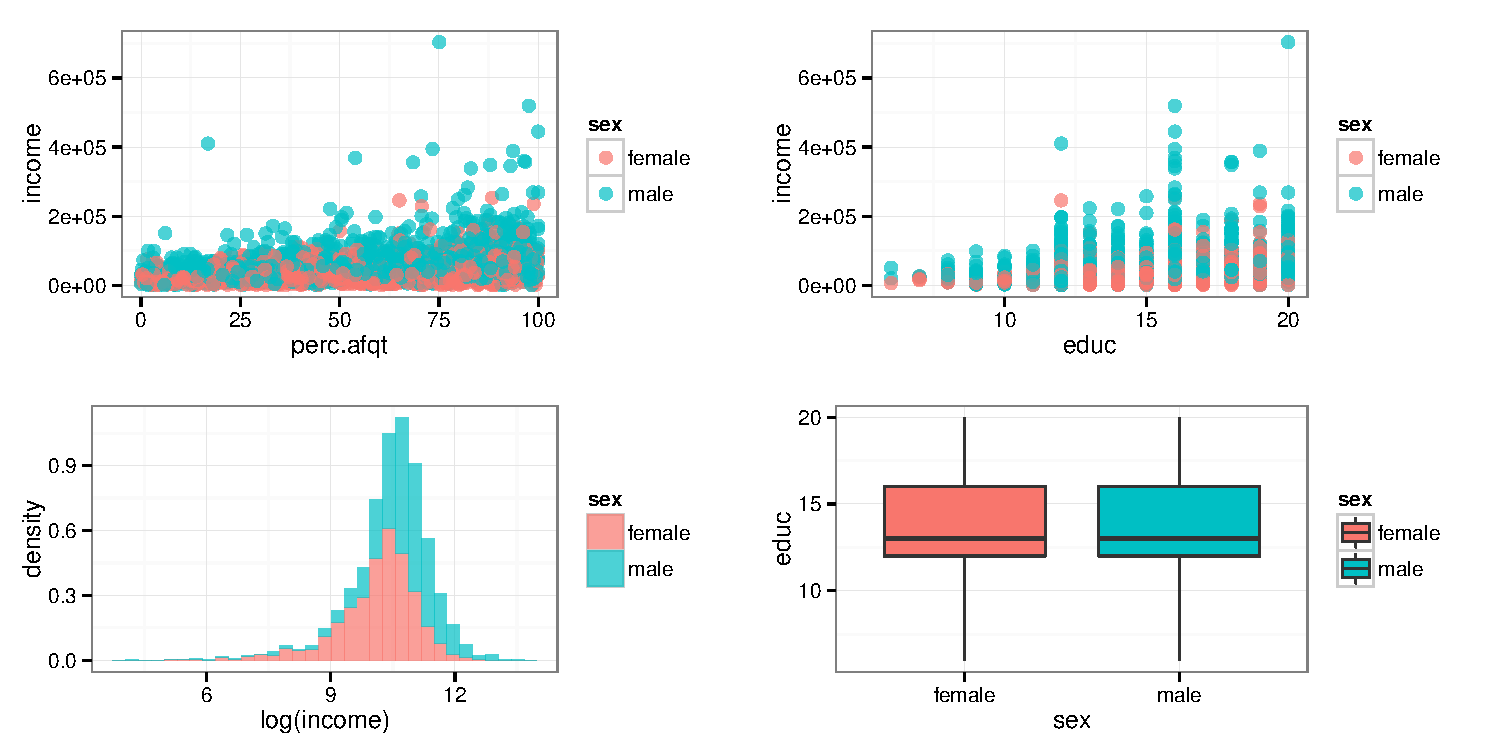
\includegraphics[width=\maxwidth]{figure/2_eda_plot-1} 

}

\caption[Esta es una gráfica exploratoria]{Esta es una gráfica exploratoria}\label{fig:2_eda_plot}
\end{figure}


\end{knitrout}

Voy a hacer una referecia a la sección \ref{sec:intro} y a la tabla \ref{tab:Tabla1} y por último a la Figura \ref{fig:2_eda_plot}. También muestro una ecuación \ref{eq:formula1}

\begin{eqnarray}
 y &=& x^4 + 4      \nonumber \\
   &=& (x^2+2)^2 -4x^2 \nonumber \\
   &\le&(x^2+2)^2
   \label{eq:formula1}
\end{eqnarray}

\end{document}
